\documentclass[a4paper,12pt]{article}
\usepackage{HomeWorkTemplate}
\usepackage{circuitikz}
\usepackage[shortlabels]{enumitem}
\usepackage{float}
\usepackage{hyperref}
\usepackage{tikz}
\usepackage{amsmath}
\usepackage{amssymb}
\usepackage{tcolorbox}
\usepackage{xepersian}
\settextfont{XB Niloofar}
\usetikzlibrary{arrows,automata}
\usetikzlibrary{circuits.logic.US}
\usepackage{changepage}
\newcounter{problemcounter}
\newcounter{subproblemcounter}
\setcounter{problemcounter}{1}
\setcounter{subproblemcounter}{1}
\newcommand{\problem}[1]
{
	\subsection*{
		پرسش
		\arabic{problemcounter} 
		\stepcounter{problemcounter}
		\setcounter{subproblemcounter}{1}
		#1
	}
}
\newcommand{\subproblem}{
	\textbf{\harfi{subproblemcounter})}\stepcounter{subproblemcounter}
}


\begin{document}
\handout
{مقدمه‌ای بر بیوانفورماتیک}
{دکتر علی شریفی زارچی - دکتر سمیه کوهی}
{نیم‌سال اول 1400\lr{-}1401}
{اطلاعیه}
{پرهام چاوشیان}
{98100118}
 {گزارش پروژه نهایی}
\textbf{مقدمه}\\
در این پروژه هدف بررسی داده‌های
$microarray$
برای بیماری
$AML$
بوده است. در پایان این گزارش به طور مفصل در مورد این بیماری توضیح داده شده است، اما به طور خلاصه این بیماری نوعی سرطان خون و مغز استخوان به حساب می‌آید که در آن سلول‌های
$meyoid$
بیش از حالت عادی تولید می‌شوند. این مشکل منچر به افزایش تولید پیش‌سازه‌های گلبول‌های سفید می‌شود که توانایی مقابله با عفونت را ندارند و بدین ترتیب بدن در برابر عفونت ضعیف می‌شود. این بیماری به کم‌خونی و کاهش تعداد گلبول‌های قرمز منجر می‌شود و در عوض آن سلول‌های خونی غیرعادی‌ای تولید می‌شوند که سبب نارسایی‌های گوناگون می‌شوند.
\par{}
در این پروژه قصد داریم تا از مجموعه داده
$GSE48558$
استفاده کنیم و ارتباط بین تغییر بیان ژن‌ها در افراد مبتلا و افراد سالم را بیابیم.\\
\textbf{تحلیل کد} \\
برای تحلیل این پروژه از زبان برنامه‌نویسی $R$ اسستفاده شده است و تمامی کدها در محیط $RStudio$ اجرا شده‌اند. برای اجرا کردن زبان $R$، از نسخه 2.1.4 این زبان استفاده شده است. در ادامه عملکرد کلی هر بخش را توضیح خواهیم داد. ابتدای هر بخش در کد با کامنتی با همان عنوان مشخص شده است.\\
بخش
$Libraries$ :
در این بخش تمامی کتابخانه‌ها مورد نیاز که برای بارگزاری دادگان، رسم نمودار، تحلیل، بررسی و محاسبه مقادیر و ... استفاده شده‌اند آورده شده است.\\
بخش
$Load Data$ :
در این بخش با استفاده از کتابخانه
$GEOquery$
داده‌های مربوط به دادگان مذکور را بارگزاری می‌کنیم. سپس با استفاده از اطلاعات داده شده، داده‌ها را با برچسب‌های $T$به معنای سرطانی و $N$ به معنی نرمال، برچسب‌گذاری می‌کنیم. این برچسب‌ها در متغیری به نام $group$ ذخیره می‌شوند.\\
بخش
$DeleteExtraSamples$ :
در این بخش داده‌هایی را که در هیچکدام از دسته‌های تست و نرمال قرار ندارند را حذف می‌کنیم، البته این عمل اختیاری است . اگر بخواهید سایر داده‌ها را هم در بررسی داشته باشید، کافی است که این تکه از کد را کامنت کنید و برنامه را اجرا کنید.\\
بخش
$Draw Boxplot$ :
در این بخش نحوه توزیع ژن‌‌ها مختلف را بررسی می‌کنیم. ابتدا اطلاعات دادگان را در یک متغیر نگه می‌داریم و سپس اندیس برچسب‌های مرتب شده را به دست می‌آوریم. در نهایت با استفاده از توابع کتاب‌خانه‌ای، نمودار زیر به دست می‌آید:
\begin{figure}[H]
 \centering
  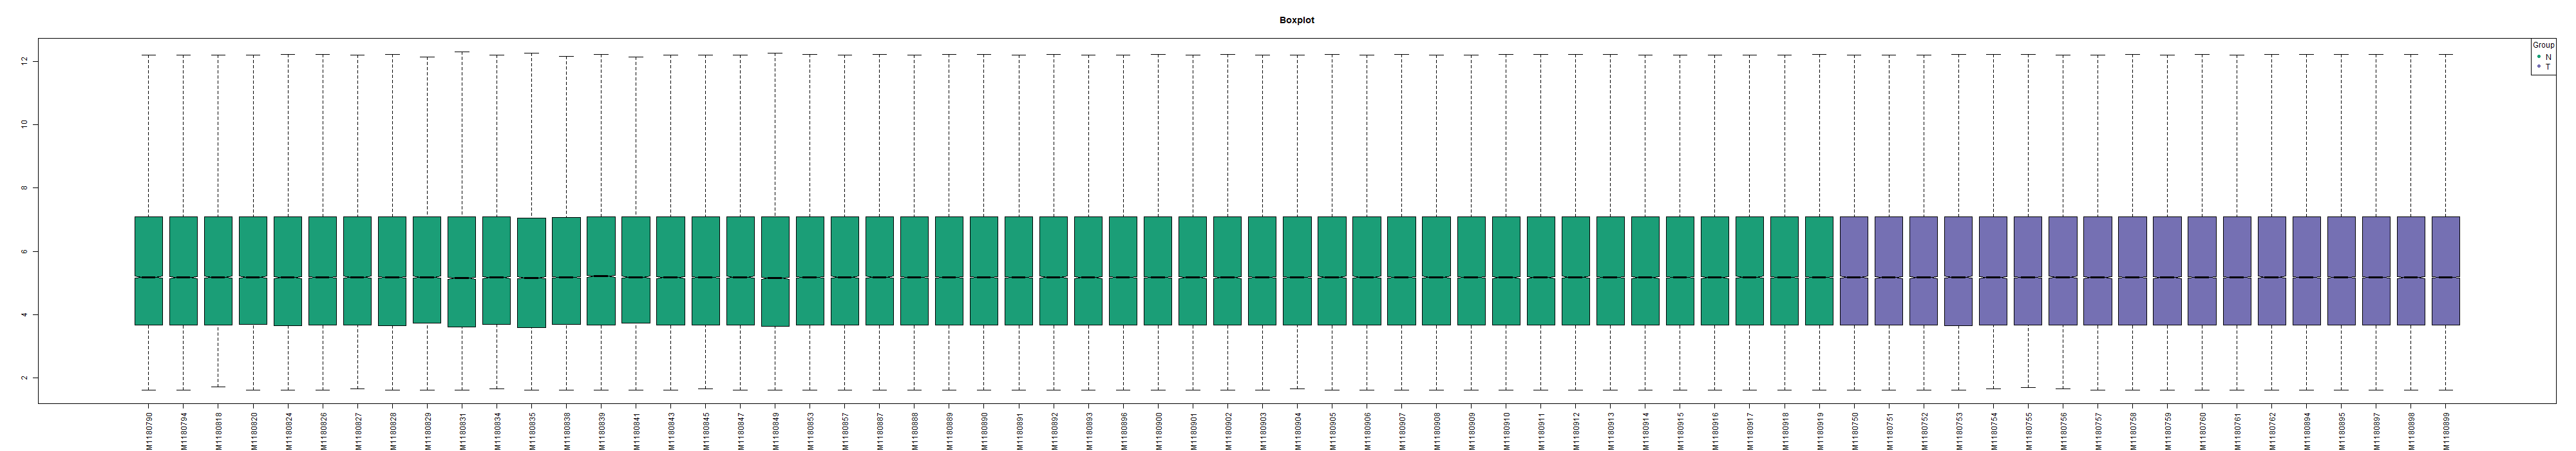
\includegraphics[width=\linewidth , height=6cm]{../../results/boxplot.png}
\end{figure}
تحلیل و بررسی شکل داده شده نشان می‌دهد که در درجه اول داده‌ها در مقیاس لگاریتمی هستند و احتیاجی به تغییر مقیاس نداریم. همچنین نزدیک بودن میانه، چارک اول و چارک سوم توزیع‌ها، نشان می‌دهد که احتیاجی به نرمالیزه کردن داده‌ها نداریم.\\
بخش
$Dimension Reduction$
در این بخش با استفاده از 3 الگوریتم متفاوت بعد داده‌های ورودی را به دو بعد کاهش می‌دهیم تا قابل ترسیم و بررسی باشند. به ازای هر الگوریتم، کد دو خروجی تولید می‌کند. یکی از آن‌ها مربوط به کاهش بعد هر $sample$ است(حالتی که ژ‌ن‌ها ویژگی باشند) و خروجی دیگر مربوط به کاهش بعد هر ژن است(حالتی که $sample$ها ویژگی باشند). خروجی دوم به صورت حاشیه‌ای تولید شده است و خروجی اصلی که ما مورد بررسی قرار می‌دهیم همان خروجی اول است.\\
الگوریتم $PCA$ : ابتدا نتیجه حاصل از این روش را می‌آوریم:
\begin{figure}[H]
 \centering
  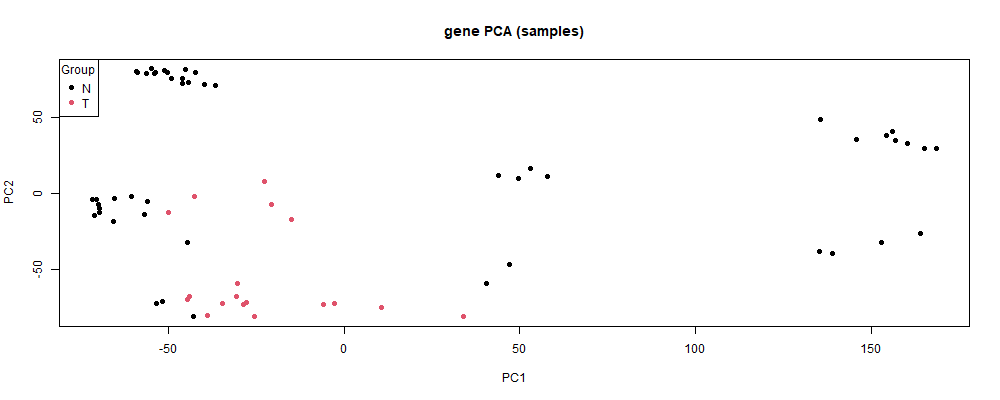
\includegraphics[width=\linewidth , height=6cm]{../../results/pca_samples.png}
\end{figure}
همانطور که در شکل مشاهده می‌شود، این الگوریتم توانسته تفکیک نسبتا خوبی از $sample$ها نرمال و تست را نشان دهد. اما همانطور که قابل مشاهده است، نمونه‌ها نرمال، در دو خوشه توزیع شده‌اند، یکی از این خوشه‌ها، بسیار نزدیک به خوشه تست است.\\
الگوریتم $tSNE$ : نتیجه حاصل شده از این روش به شکل زیر است:
\begin{figure}[H]
 \centering
  \includegraphics[width=\linewidth , height=6cm]{../../results/tsne_samples.png}
\end{figure}
این الگوریتم در جداسازی داده‌ها نسبت به الگوریتم قبلی، غملکرد بهتری داشته است، اما مشاهده می‌شود که سه تا از نمونه‌های نرمال همچنان در نزدیکی این نمونه‌ها تست قرار گرفته‌اند و بالعکس؛ که می‌توان اینطور برداشت کرد که این نمونه‌ها در ابعاد بالا نیز نزدیک به نمونه‌های گروه مقابل شبیهند.\\
الگوریتم $UMAP$ : نتیجه حاصل شده از این روش به شکل زیر است:
\begin{figure}[H]
 \centering
  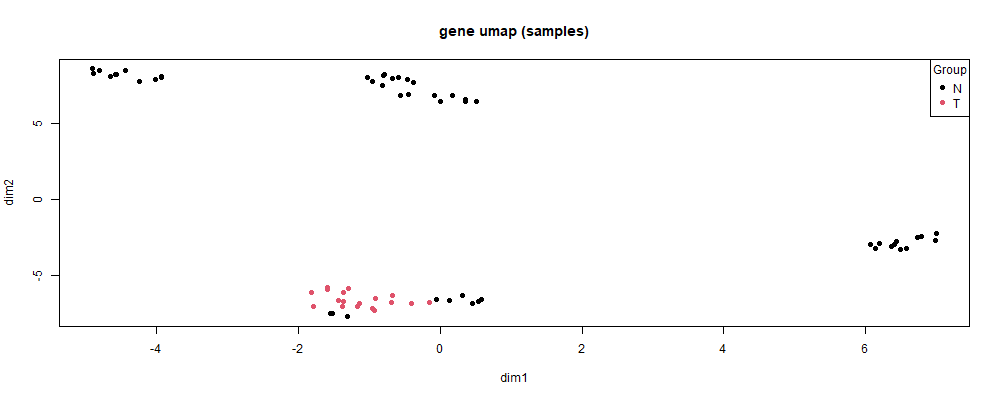
\includegraphics[width=\linewidth , height=6cm]{../../results/umap_samples.png}
\end{figure}
در این الگوریتم، فاصله‌ای که بین خوشه‌های تست و نرمال افتاده است، به نسبت دو الگوریتم قبلی بیشتر است، اما تعداد نمونه‌ها نرمال که در بین نمونه‌های تست قرار گرفته‌اند، از الگوریتم $tSNE$ بیشتر است.\\
بنا به توضیحات داده شده، ما در ادامه برای کاهش ابعاد، از الگوریتم $tSNE$ استفاده می‌کنیم.\\
بخش
$Correlation$ :
در این بخش همسبتگی نمونه‌ها را با استفاده از دو $heatmap$ بررسی می‌کنیم:
\begin{figure}[H]
 \centering
  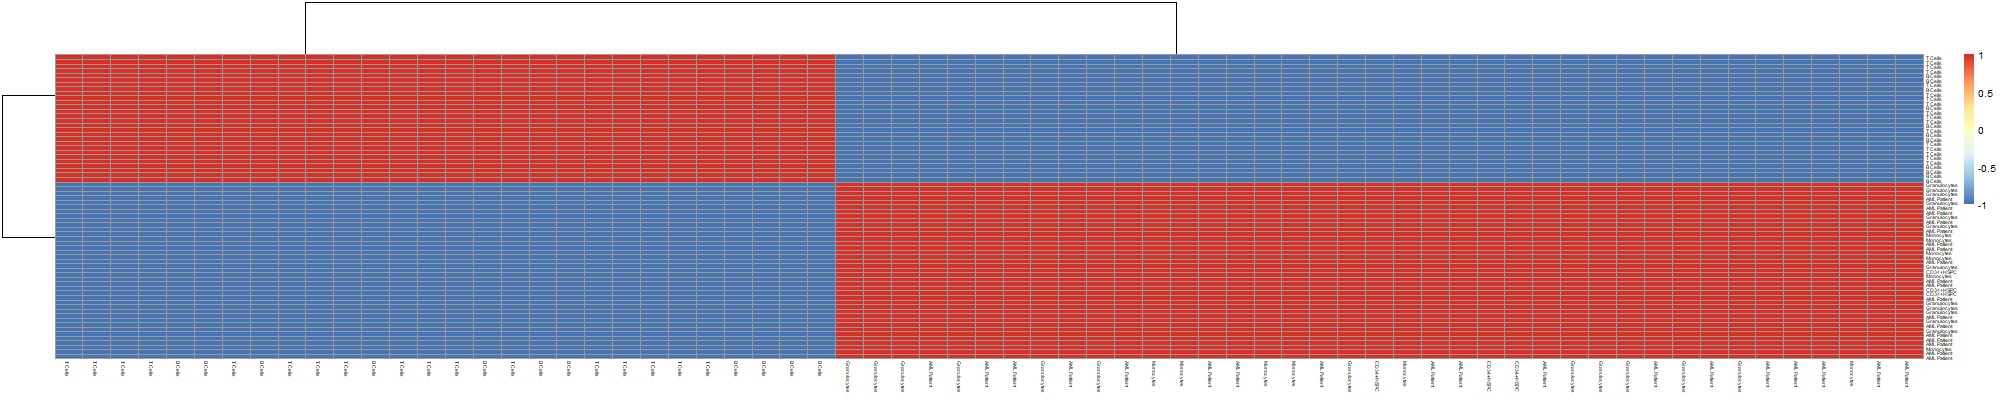
\includegraphics[width=\linewidth , height=12cm]{../../results/heatmap_reducted.png}
\end{figure}
\begin{figure}[H]
 \centering
  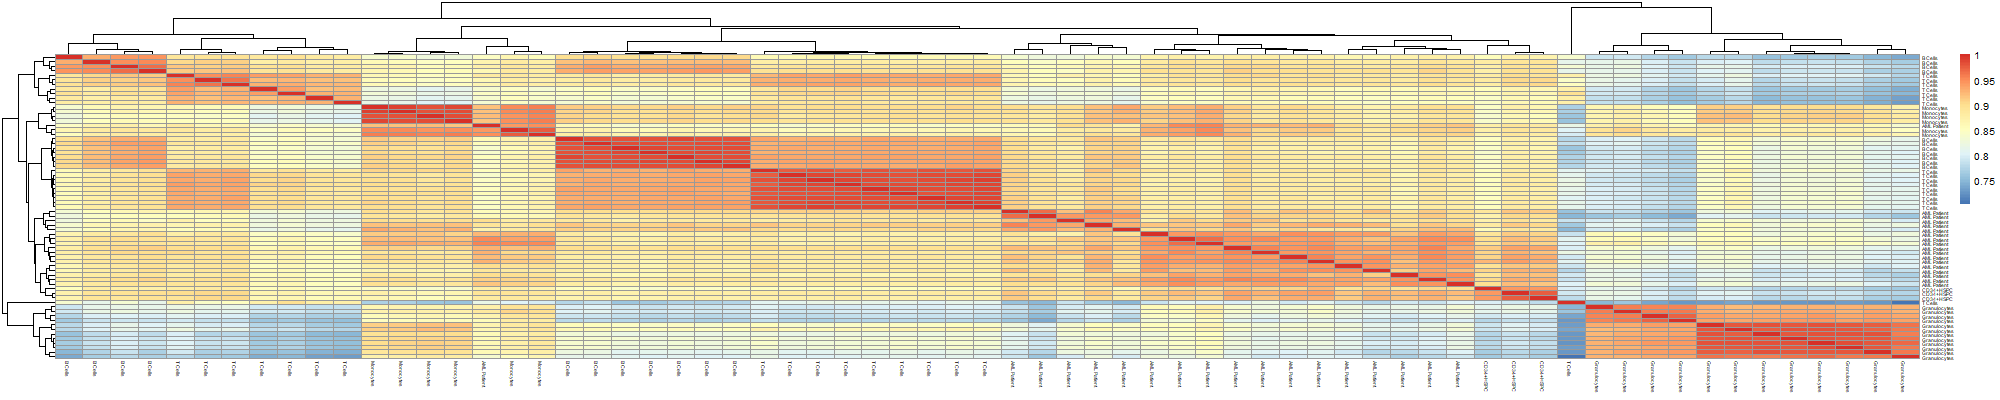
\includegraphics[width=\linewidth , height=12cm]{../../results/heatmap.png}
\end{figure}
نمودار اول با استفاده از داده‌ها کاهش بعد یافته در قسمت قبل به دست آمده است، همانطور که مشاهده می‌شود، این نمودار اطلاعات مفید زیادی به ما نمی‌دهد. بنابراین تصمیم گرفتیم که از داده‌های اصلی نیز برای ساختن یک $heatmap$ دیگر استفاده کنیم که حاصل آن شکل دوم شده است. همانطور که مشاهده می‌شود این شکل به خوبی روابط همبستگی بین نمونه‌ها را نشان می‌دهد و مقادیر آن صرفا 1 یا منفی 1 نیستند. بر طبق این جدول بیشترین همبستگی منابع به تست، به ترتیب $monocytes$ و $cd34$ هستند.\\
بخش:
$Differential Expression Analysis$ :
در ابتدای این بخش ماتریسی می‌سازیم که با استفاده از آن نمونه‌ها به صورت
$OneHot$
برچسب‌گذاری می‌شوند. از این ماتریس در ادامه استفاده خواهیم کرد. سپس با استفاده از توابع کتابخانه
$limma$
یک ماتریس که به نوعی بیانگر اختلاف بین نمونه‌ها با برچسب‌های متفاوت است به دست می‌آوریم و
یک مدل خطی برروی داده فیت می‌کنیم. برای اینکه بتوانیم از توزیع‌ پیشین در مدلمان استفاده کنیم، یک مدل بیزی جدید با استفاده از مدل قبلی بر روی داده‌ها فیت می‌کنیم. در نهایت جدولی به دست می‌آید که شامل اطلاعات زیادی در مورد ژن‌ها است اما از بین تمامی اطلاعات ما تنها نام و نشانه ژن،
$Adj\;P\;Value$
و
$logFC$
را نگه می‌داریم. تفاوت معنادار را به این صورت تعیین کرده‌ایم که میزان بیان حداقل دو برابر یا حداکثر نصف شده باشد و از طرفی هم در بین ژن‌ها با این ویژگی، آن‌هایی که
$Adj\;P\;Value$
کمتر از 5 درصد است را نگه‌ می‌داریم. ژن‌های به دست آمده را در دو فایل ذخیره می‌کنیم. برخی از ژن‌ها ممکن است دارای چند نام باشند، نام‌های مختلف آن‌ها را در سطور مختلف می‌نویسیم.\\
\textbf{آنالیز $gene\; ontology$ و $pathway$ها}: \\
ابتدا لازم به ذکر است که به علت کثرت ژن‌ها، 100 ژن ابتدایی برای تحلیل به سایت
\href{https://maayanlab.cloud}{Enrichr}
داده شده‌اند.\\
ژن‌ها با بیان بالاتر: بر طبق خروجی ساید مذکور، بر اساس 3 مجموعه
$BioPlane\; 2019$
،
$KEG; 2021\; Human$
و
$Elsevie; Pathway\; Collection$
در میان $pathway$ها،
$Cell\; cycle$
بیشتر مورد توجه بوده است، که تصویر آن در ادامه آمده است.
\begin{figure}[H]
 \centering
  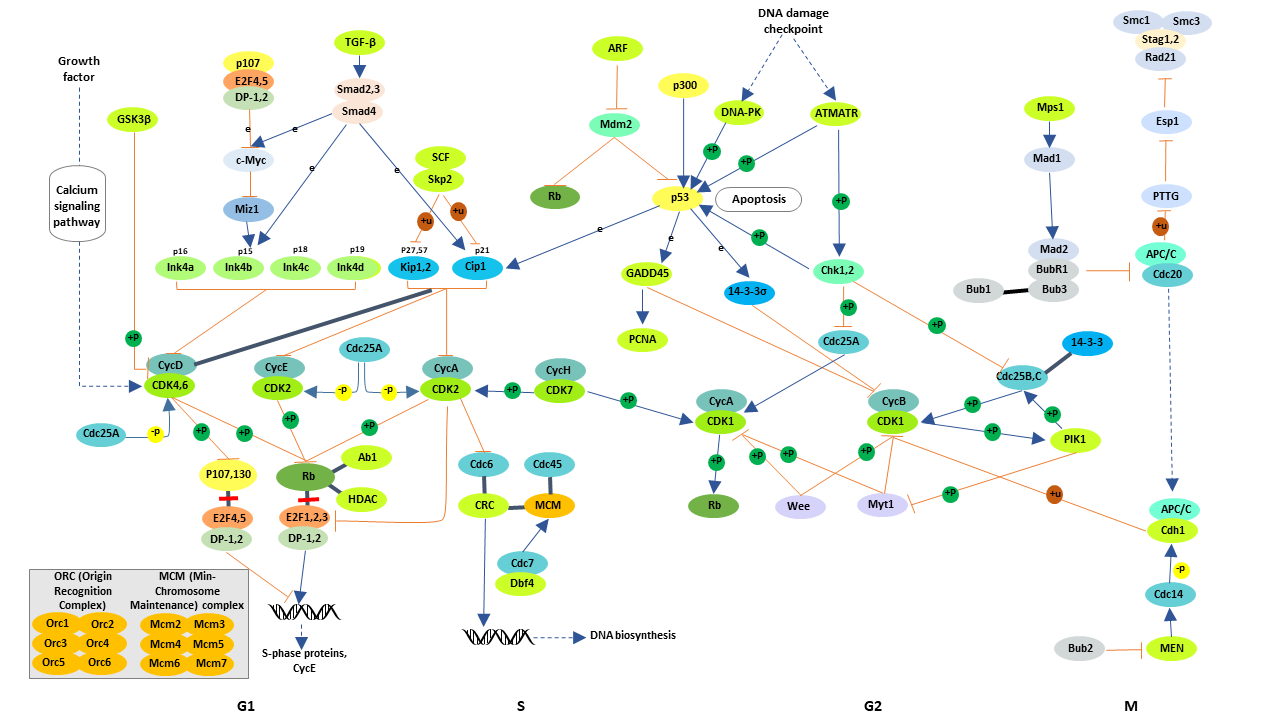
\includegraphics[width=0.8\linewidth , height=6cm]{../../source/Cell-cycle-picture.png}
\end{figure}

بر اساس مجموعه
$WikiPathway\; 2021\; Human$
،
$Retinoblastoma\;gene\; in\; cancer\; WP2446$
مورد توجه‌ترین $pathway$ بوده است
که تصویر آن را در ادامه مشاهده می‌نمایید.
\begin{figure}[H]
 \centering
  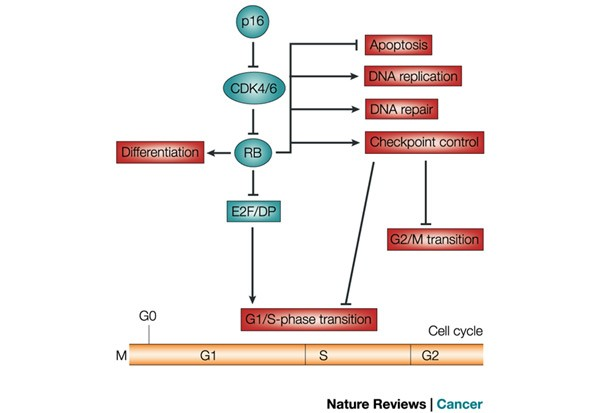
\includegraphics[width=0.8\linewidth , height=6cm]{../../source/cancer.jpg}
\end{figure}
نتایج به دست آمده مورد انتظار هم بودند، چرا که هنگام ابتلا به سرطان، چرخه سلولی تحت تاثیر قرار می‌گیرد.\\
در زمینه تحلیل $ontology$ها، در سه زمینه زیر موارد قابل توجه را بیان می‌کنیم:\\
زمینه
$Biological\; Process$ : 
طبق
$GO\; Biological\; Process\; 2021$
موارد زیر در این زمینه قابل توجه‌اند:
\begin{latin}
\begin{itemize}
\item mitotic spindle organization (GO:0007052)
\item DNA metabolic process (GO:0006259)
\item microtubule cytoskeleton organization involved in mitosis (GO:1902850)
\end{itemize}
\end{latin}
زمینه
$Molecular\; Function$ : 
طبق
$GO\; Molecular\; Function\; 2021$
موارد زیر در این زمینه قابل توجه‌اند:
\begin{latin}
\begin{itemize}
\item DNA replication origin binding (GO:0003688) (GO:1902850)
\item microtubule motor activity (GO:0003777)
\item motor activity (GO:0003774)
\end{itemize}
\end{latin}
زمینه
$Cellular\; Component$ : 
طبق
$GO\; Cellular\; Component\; 2021$
موارد زیر در این زمینه قابل توجه‌اند:
\begin{latin}
\begin{itemize}
\item nucleus (GO:0005634)
\item spindle (GO:0005819)
\item intracellular membrane-bounded organelle (GO:0043231)
\end{itemize}
\end{latin}
حال به بررسی ژن‌ها با بیان پایین‌تر می‌پردازیم:\\
ژن‌ها با بیان پایین‌تر: برخلاف قسمت قبل، مسیری که اکثریت مجموعه‌ها در اولویت اول قرار دهند وجود نداشت. برای مجموعه
$BioPlanet\; 2019$
مورد توجه‌ترین مسیر
$Interleukin-2\; signaling\; pathway$
بوده است و برای مجموعه
$KEGG\; 2021\; Human$
مورد توجه‌ترین مسیر
$Sphingolipi; signaling\; pathway$
بوده است.
\\
مجددا در زمینه تحلیل $ontology$ها، در سه زمینه زیر موارد قابل توجه را بیان می‌کنیم:\\
زمینه
$Biological\; Process$ : 
طبق
$GO\; Biological\; Process\; 2021$
موارد زیر در این زمینه قابل توجه‌اند:
\begin{latin}
\begin{itemize}
\item positive regulation of type I interferon-mediated signaling pathway (GO:0060340)
\item positive regulation of innate immune response (GO:0045089)
\end{itemize}
\end{latin}
زمینه
$Molecular\; Function$ : 
طبق
$GO\; Molecular\; Function\; 2021$
موارد زیر در این زمینه قابل توجه‌اند:
\begin{latin}
\begin{itemize}
\item TAP1 binding (GO:0046978)
\end{itemize}
\end{latin}
زمینه
$Cellular\; Component$ : 
طبق
$GO\; Cellular\; Component\; 2021$
موارد زیر در این زمینه قابل توجه‌اند:
\begin{latin}
\begin{itemize}
\item phagocytic vesicle membrane (GO:0030670)
\end{itemize}
\end{latin}
\begin{center}
\line(1,0){450}
\end{center}
\textbf{توضیحاتی درباره $AML$}\\
$AML$
در واقع اختصاری برای
$Acute\; Myeloid\; Leukemia$
،
بنابراین بهتر است پیش از آنکه درباره $AML$ توضیح دهیم، بررسی کنیم که لوکمی چیست. به طور کلی، به تمامی سرطان‌هایی که در سلول‌هایی که قرار است به سلول خونی منجر شوند ایجاد می‌شود، لوکمی می‌گویند. رایج‌ترین شکل لوکمی در در حالات اولیه سلول‌های سفید خونی مشاهده می‌شود، اما این مسئله در سایر سلول‌ها نیز مشاهده شده است. لوکمی‌ها ممکن است در سلول‌‌های مغز استخوان یا لنفاوی ایجاد شوند. همچنین بر اساس سرعت رشد، لوکمی‌ها به دو دسته مزمن و حاد تقسیم می‌شوند.\\
$AML$
لوکمی حاد مغز استخوان است، که در بافت مغز استخوان آغاز می‌شود. $AML$ها اکثرا به سرعت به خون منتقل می‌شوند و همچنین در موارد حادتر، به بخش‌های دیگر بدن مانند:مغز و نخاع، کبد و گره‌های لنفائی متاستاز می‌دهند.\\
برخی عوامل افزایش احتمال ابتلا به $AML$:\\
در اینجا چند مورد از مواردی که سبب افزایش احتمال ابتلا به $AML$ می‌شوند را بررسی می‌کنیم:
\begin{itemize}
\item سن : احتمال ابتلا به این بیماری رابطه مستقیمی با سن فرد دارد و با افزایش سن، احتمال ابتلا نیز افزایش می‌یابد.
\item جنسیت : طبق آمار، ابتلا به $AML$ در مردان شایع‌تر از زنان است.
\item استعمال دخانیات : استعمال دخانیات می‌تواند احتمال ابتلا به $AML$ را (همانند بسیاری بیماری دیگر) افزایش دهد.
\item مواد شیمیایی : قرار گرفتن در معرض برخی مواد شیمیایی مانند، مانند بنزن، می‌تواند احتمال ابتلا را افزایش دهد.
\item مواد رادیواکتیو : قرار گرفتن در معرض پرتوهای رادیواکتیو می‌تواند ریسک ابتلا را افزایش دهد.
\item سابقه خانوادگی : احتمال ابتلا در افرادی که ساقه این بیماری را در خانواده خود داشته‌اند بیشتر است.
\end{itemize}
علائم مبتلا شدن به بیماری $AML$ : \\
این بیماری علائم مختلفی دارد که می‌توان آن‌ها را به چند دسته تقسیم کرد:\\
دسته علائم عمومی: علائم زیر در بین بیمارن $AML$ شایعند، البته به ذکر است که این علائم به $AML$ منحصر نیستند و تنها نمی‌توان به همین علائم برای تشخیص اکتفا کرد:
\begin{itemize}
\item خستگی
\item کاهش اشتها
\item کاهش وزن
\item تب
\item عرق‌های شبانه
\end{itemize}
دسته علائم ناشی از افزایش سلول‌های لوکمی: سلول‌ها لوکمی به طور متوسط از سول‌ها خونی نرمال بزرگترند. این موضوع منجر به این می‌شود که تعداد زیادی از آن‌ها سبب ایجاد لخته خونی و انسداد رگ بشوند. که ممکن است این موضوع به سکته هم منجر شود، در این صورت به این بیمار باید به طور اورژانسی رسیدگی شود. به این وضعیت $Leukostasis$ گفته می‌شود که از جمله علائم آن به شرح زیر است:
\begin{itemize}
\item تکلم گنگ
\item ضعف در یک سمت بدن
\item گیجی
\item سردرد
\item خواب آلودگی
\end{itemize}
دسته علائم مربوط به کاهش سلول‌های خونی قرمز: کاهش این سلول‌ها در بدن علل مختلفی دارد، اما یکی از علل آن، ابتلا به $AML$ است. از علائم آن می‌توان به موارد زیر اشاره کرد:
\begin{itemize}
\item خستگی
\item ضعف
\item سردرد
\item سرگیجه
\item تنگی نفس
\item احساس لرز
\item رنگ‌پریدگی
\end{itemize}
دسته علائم مربوط به کاهش سلول‌های خونی سفید نرمال: از آنجایی که این سلول‌ها مسئول محافظت از بدن در برابر بیماری‌ها و عفونت‌ها هستند، بنابراین در صورت کاهش آن‌ها، مشکلات عفونی در کوتاه‌مدت بهبود نمی‌یابند و فرد در فواصل زمانی کوتاهی دچار مشکل می‌شود. البته لازم به ذکر است که در صورت ابتلا به $AML$ ممکن است نه تنها شخص دچار کاهش سلول سفید نشود، بلکه این سلول‌ها افزایش هم پیدا کنند، اما همگی آن‌ها غیر نرمال و در دفاع از بدن بی‌تاثر هستند.\\
دسته علائم مربوط به کاهش پلاکت: کمبود پلاکت به شکل‌ها زیر می‌تواند خودش را بروز دهد:
\begin{itemize}
\item خونریزی‌ها شدید و مکرر بینی
\item خونریزی لثه
\item خونرریزی‌های طولانی به طوری که خون بند نیاید
\item کبودی در نواحی مختلف پوست
\end{itemize}
دسته علائم شرایط حاد بیماری و انتشار آن به سایر بخش‌ها بدن:
\begin{itemize}
\item صرع
\item مشکل در تعادل
\item تاری دید
\item بی‌حسی صورت
\item ضعف
\item سردرد
\item تهوع و استفراغ
\end{itemize}
علل بروز بیماری $AML$:\\
بع طور کلی در هر سلول، ژن‌هایی وجود دارند که مسئول تکثیر و مرگ سلولند. به ژن‌های مسئول رشد و تکثیر سلول، $Oncogene$ و به ژن‌ها مسئول مرگ و میر سلول،
$Tumor\; Suppressor\; Gene$
گفته می‌شود. گاهی اوقات در فرایند تکثیر سلول، ممکن است این ژن‌ها دچار تفییر شوند به گونه‌ای که ژن‌های تکثیر بیش از حد فعال شوند یا ژن‌های مرگ غیرفعال شوند. در چنین شرایطی است که رشد و تکثیر سلول از حالت عادی خارج شده و به تومور و سرطان منجر می‌شود. تغییرات رخ داده ممکن است به شکل‌های جابه‌جایی، حذف یا معکوس شدن کروموزوم باشند.\\
برخی ژن‌های مهم در ابتلا به $AML$:\\
طبق تحقیقات از جمله ژن‌های مهم در بیماری $AML$، ژن‌های $FLT3$ و $KIT$ هستند که در میان ژن‌ها با بیان بالاترو در نتایج ما، به ترتیب در رتبه‌های 2 و 20 ظاهر شده‌اند. البته برخی ژن‌ها نیز مانند ژن $CEBPA$ و $NPM1$ که بنابر تحقیقات مهم خوانده شده‌اند اما در میان نتایج ما در رتبه‌های پایین قرار گرفته‌اند. برای اطلاعات تکمیلی می‌توانید به این
\href{https://www.ncbi.nlm.nih.gov/pmc/articles/PMC5767295/#:~:text=Recently%2C%20with%20the%20development%20of,%2C%20ASXL1%2C%20PTPN11%20and%20CBL.}{لینک}
مراجعه کنید.\\
درمان بیماری $AML$:\\
یکی از داروهایی که در بزرگسالان برای درمان این بیماری استفاده می‌شود
$XOSPATA$
است. این دارو برروی ژن
$FLT3$
که بالاتر در مورد آن صحبت شد اثرگذار است. برای اطلاعات بیشتر این
\href{https://www.xospata.com/?gclid=Cj0KCQiAgP6PBhDmARIsAPWMq6n3jJhNQjcKUpJGAGSPHgIlPkbCdjJn69pUDozbftPdSNqCMeMxLqEaAsE2EALw_wcB&gclsrc=aw.ds}{لینک}
را مطالعه کنید. همچنین در این
\href{https://www.cancer.gov/about-cancer/treatment/drugs/leukemia#3}{لینک}
می‌توانید لیستی از داروهایی که برای درمان $AML$ کاربرد دارند را مشاهده کنید.
\end{document}